\subsection{Canal binário simétrico em cascata}

\begin{questions}

\question{
  Considere os canais binários simétricos conectados em cascata com um codificador entre
  eles, conforme ilustrado abaixo. Calcule a capacidade do canal entre $X$ e $Y$. 

  \begin{figure}[h!]
  \centering
  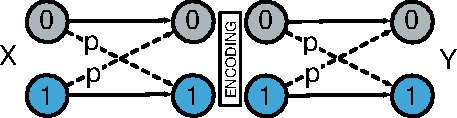
\includegraphics[width=0.5\textwidth]{../images/c-enc-c.pdf}
  \label{fig:c-enc-c}
  \end{figure}

  Qual é a capacidade deste canal?
}
\begin{solution}
  Os símbolos são re-codificados após o primeiro canal, desta forma a
  capacidade torna-se $C = \min (C_1, C_2)$, onde $C_1$ e $C_2$ são as
  capacidades do primeiro e segundo canais binários, respectivamente.
  Como neste caso os canais são iguais, temos $C_1 = C_2 = 1 - H(p)$.
  Logo, a capacidade do canal será $C = 1 - H(p)$, sendo este valor alcançado
  quando a distribuição de $X$ for uniforme.
\end{solution}


\question{
Considere um canal formado por dois canais binários simétricos em casacata,
conforme ilustrado abaixo. Calcule a capacidade deste canal.

\begin{figure}[h]
\centering
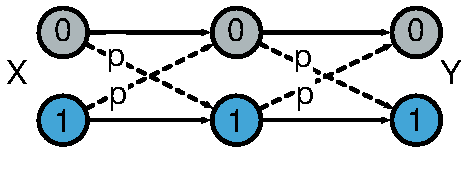
\includegraphics[width=0.3\textwidth]{../images/bscc.pdf}
\end{figure}


}
\begin{solution}
O canal total terá a seguinte matriz de transmissão:
\begin{equation}
p(y|x) = 
\begin{pmatrix}
(1-p)^2 + p^2 & 2p (1-p) \\
2p (1-p)      & (1-p)^2 + p^2
\end{pmatrix}
\end{equation}


A capacidade do canal é dada por:
\begin{align}
C &= \max_{p(x)} I(X;Y) = \max_{p(x)} \left( H(Y) - H(Y|X) \right) \nonumber \\
  &= 1 - H\left( (1-p)^2 + p^2, 2p (1-p) \right) = 1 - H\left( 2p (1-p) \right) \nonumber \\
  &= 1 + \left((1-p)^2 + p^2\right) \log \left( (1-p)^2+p^2 \right) + 2p (1-p) \log \left( 2p(1-p) \right) \nonumber \\
  &= \left(1 - H(p)\right)^2
\end{align}

Faça a verificação numérica do último passo para $p \in [0,1]$.

Ou confira o resultado no \href{https://www.wolframalpha.com/input/?i=1+%2B+%28%281-p%29%5E2%2Bp%5E2%29+%5Clog+%28%281-p%29%5E2%2Bp%5E2%29+%2B+2p%281-p%29+%5Clog%282p%281-p%29%29++-+%281+%2B+p+%5Clog+p+%2B+%281-p%29%5Clog+%281-p%29%29%5E2}{WolframAlpha}.


\end{solution}
\end{questions}
